%%%%%%%%%%%%%%%%%%%%%%%%%%%%%%%%%%%%%%%%%%%%%%%%%%%%%%%%%%%%%%%%%%%%%%%%%%%%
% Design Process
%%%%%%%%%%%%%%%%%%%%%%%%%%%%%%%%%%%%%%%%%%%%%%%%%%%%%%%%%%%%%%%%%%%%%%%%%%%%

\chapter{Design Process}
\label{chapter:design_process}
The development of SoleMate was guided by a structured design process shaped by both technical and non-technical constraints. Throughout this project, multiple constraints influenced the selection of system components, overall architecture, and design. As a result, multiple design alternatives were evaluated. Based on these insights, key design conditions were defined and refined during subsequent iterations to ultimately achieve a reliable and functional prototype. Relevant engineering standards were considered to ensure that the system met essential requirements. 

%In this chapter, you should discuss in detail the entire design process that you have adopted at the end of EECE 501 and throughout the entire scope of EECE 502. Accordingly, you need to:
% \begin{itemize}
%     \item Outline the constraints that you have identified to achieve your project
%     \item Discuss the various design alternatives that you have identified 
%     \item Specify the design decisions that you have made based on the identified constraints and engineering requirements.
%     \item Clearly outline the different design iterations you have gone through to have your final product fully functional
%     \item Show how the engineering standards are used as part of the design decision process
% \end{itemize}

%\textbf{Accordingly, this chapter must be composed of five main sections.} 

\section{Engineering Constraints}
As SoleMate is a real-world wearable system, it was influenced and shaped by multiple factors, such as technical constraints and non-technical constraints. These factors directly influenced sensor selection, system architecture, and ML deployment. The design process was guided by the balance of trade-offs and limitations.\\

\subsection{Technical Constraints}
The technical constraints for SoleMate arise directly from the hardware architecture, sensing modalities, and real-time processing requirements of the system.\\

\begin{itemize}
    \item \textbf{Limited Microcontroller Resources}\\
    The Arduino Nano 33 BLE imposes strict constraints on processing speed, available memory, and the number of tasks that can run in parallel. These limitations prevent onboard execution of the CapsNet and Spectro-Temporal models. Firmware must therefore remain lightweight while still handling sensor polling, BLE packet construction, and AES-128 encryption simultaneously.
    \item  \textbf{Physical Wiring and Pin Limitations}\\
    The chosen microcontroller, Arduino Nano 33 BLE, contains 14 digital Input/Output (I/O) pins and 8 analog I/O pins, shared with the digital pins. With multiple sensors requiring interfacing, the limited number of General Purpose Input/Output (GPIO) pins must be distributed across all sensors. This limitation necessitates the use of techniques such as multiplexing to connect multiple sensors.
    \item \textbf{Plantar Pressure Matrix Cross-Talk}\\
    The Velostat-based resistive sensing matrix is inherently susceptible to cross-talk, where current from one sensing node leaks into adjacent rows or columns, producing ghost pressure readings at unloaded nodes. This directly degrades the spatial accuracy of the plantar heatmaps used as input to the CapsNet ataxia classifier. This limitation introduces errors and requires mitigation strategies.
    \item \textbf{PPG Signal Quality at the Foot}\\
    Placing the MAX30102 sensor on the foot rather than the fingertip or wrist significantly increases susceptibility to motion artifacts and poor perfusion. The pulsatile AC component of the PPG signal can be corrupted during walking, making it difficult to reliably extract the waveform features required for blood pressure estimation. This constraint requires signal processing and quality control mechanisms. 
    \item \textbf{BLE Throughput and Latency}\\
    The system must transmit four concurrent data streams, plantar pressure frames, PPG samples, flex sensor readings, and IMU data, over a single BLE connection at rates sufficient for real-time visualization. BLE packet size limits and connection interval constraints impose an upper bound on achievable throughput, necessitating optimized data transmission strategies to avoid data loss or excessive latency in the Android application.
    \item \textbf{Power Consumption and Battery Life}\\
    Continuous simultaneous operation of the Velostat multiplexer array, the MAX30102, four flex sensors, the onboard IMU, AES-128 encryption, and BLE radio places a substantial load on the 3.7~V Li-Po battery. Careful power management strategies are necessary to achieve a useful operating duration without increasing the battery size beyond what is practical for a foot-worn device.
    \item \textbf{Flex Sensor Mechanical Drift}\\
    Repeated bending cycles cause the resistance baseline of the flex sensors to shift over time, introducing drift into the ankle circumference measurements used for edema classification. This introduces the need for recalibration at the start of each session and limits the long-term repeatability of the swelling severity scores without additional compensation mechanisms.
    \item \textbf{Dataset Size and Model Generalizability}\\
    The CapsNet ataxia classifier was trained on a dataset of 226 plantar pressure images from 105 subjects, which is relatively small for a deep learning model. This constrains the model's ability to generalize across different foot sizes, shoe types, and walking styles. The Spectro-Temporal blood pressure model similarly depends on MIMIC-BP data that may not reflect the population variability encountered in deployment.
\end{itemize}

\subsection{Non-Technical Constraints}
Non-technical constraints arise from considerations related to cost, usability, accessibility, and ethical obligations, particularly within the healthcare context of Lebanon. These constraints play a significant role in shaping the design decisons of the system, as they directly influence practicality, user adoption, and overall feasibility of the project in real-world applications.

\begin{itemize}
    \item \textbf{Economic Constraints and Local Procurement}\\
    Lebanon's economic conditions directly limited component sourcing throughout the project. Several sensors, including the Velostat sheet and charging module, were unavailable locally and had to be imported, incurring high shipping costs and delays. The total hardware budget was constrained to approximately \$200--250, which influenced component selection and restricted the use of higher-performance alternatives such as the Analog Devices ADPD108x medical-grade PPG sensor.
    \item \textbf{Comfort and Wearability}\\
    The device must be worn on the foot for extended periods without causing discomfort or altering the patient's natural gait. Any change in walking pattern would degrade the plantar pressure data used for ataxia classification. This constrained the form factor and limited the placement options for rigid components such as the microcontroller and battery pack.
    \item \textbf{Fit Across Patient Populations}\\
    SoleMate targets patients with multiple sclerosis and related neurodegenerative conditions, a population with variable foot geometry, potential edema-related swelling, and gait abnormalities. The sensing layout must accommodate this variability without requiring custom fabrication per patient. This introduced design constraints on the sensing area coverage and elastic band sizing.
    \item \textbf{Privacy, Consent, and Ethical Obligations}\\
    All subsystem testing involving human subjects required informed verbal and written consent from participants. The physiological data collected by SoleMate, including plantar pressure patterns, heart rate, SpO\textsubscript{2}, and blood pressure estimates, is sensitive health information. This necessitated secure data handling methods and data protection mechanisms. Ethical considerations also constrained the team's ability to collect large patient datasets locally, contributing to the reliance on public datasets such as MIMIC-BP and the Danacı et al.\ plantar pressure dataset.
    \item \textbf{Maintenance and Recalibration Requirements}\\
    The flex sensors require personalized baseline calibration at the start of each session, and the Velostat matrix requires a no-load reference frame to suppress static offsets. For a device intended for use by patients at home without clinical supervision, this creates a practical burden. The calibration procedures must therefore be simple enough to be completed by a non-technical user through the Android application without assistance.
    \item \textbf{Regulatory and Clinical Validation Constraints}\\
    SoleMate is not a certified medical device and is therefore limited to research and screening use. The blood pressure estimation model does not yet meet AAMI clinical validation criteria, and the ataxia classifier has not been validated on locally collected patient data from Lebanon. These constraints define the boundary of the system's current claims and prevent it from being used for formal clinical diagnosis within the scope of this project.
    \item \textbf{Regional Instability and Supply Chain Disruptions}\\
    Regional instability in Lebanon and the surrounding area introduced additional logistical constraints on the project. These conditions affected supply chain reliability and made it impractical to rely on external fabrication services. As a result, options such as custom flexible PCB fabrication were not pursued, as delivery timelines could not be guaranteed within the project schedule. This limitation constrained hardware design choices and reduced the opportunity for more compact and optimized implementations.
    \end{itemize}

\section{Design Alternatives}
The design process went through multiple stages of exploration and refinement. Initially, we gathered needs addressing different clinical and user preferences, as documented in Appendix D. This chapter outlines the reasoning behind each iteration and how these decisions shaped the final prototype. 

\subsection{Design Alternative 1: Clinical Mat}
During the beginning of the design process, the main goal was to detect ataxia objectively. Clinically, ataxia is still commonly assessed through visual tests and patient experience. Hence, creating a plantar pressure mat, as shown in Fig.~\ref{fig:Mat}, was considered a plausible idea. The patient would visit the clinician and walk on the mat. After a set amount of time, the clinician would be able to observe the results of the trial run and detect ataxia objectively and quickly.\\

However, although this design enables objective detection of ataxia, the sporadic nature of clinical visits would still lead to delayed detection. Consequently, this limitation motivated the consideration of Design Alternative 2.

\begin{figure}[H]
    \centering
    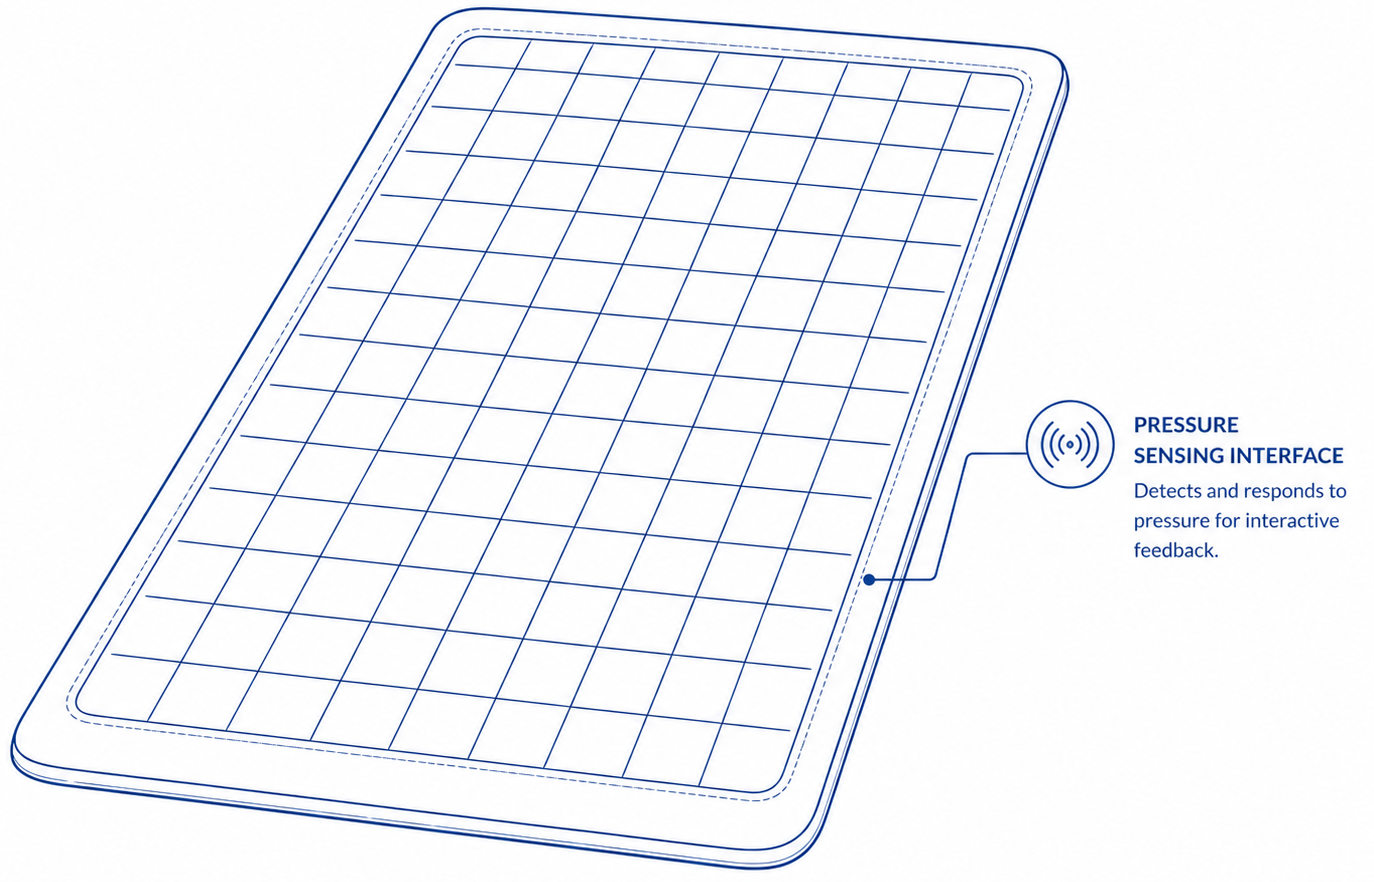
\includegraphics[width=0.75\textwidth]{FYP_Template_Spring/Figures/Mat.png}
    \caption{Initial Design of Alternative 1}
    \label{fig:Mat}
\end{figure}

\subsection{Design Alternative 2: Wearable L}
Since early detection of ataxia is crucial, a wearable design was opted for. Since the design became wearable, other biological markers from the foot could be detected. The feasibility of placing numerous sensors to detect a multitude of diseases was discussed, along with noninvasive glucose sensing, sweat analysis, heart rate, SpO$_2$, plantar pressure, movement, etc. As a result, the design seen in Fig.~\ref{fig:L} came into place. \\

However, the main concern is always the patient. Although this comprehensive super-sensor could be created, it would be ineffective if the bulky design decreased patient compliance. Thus, Design Alternative 3 was considered.
    
    \begin{figure}[H]
        \centering
        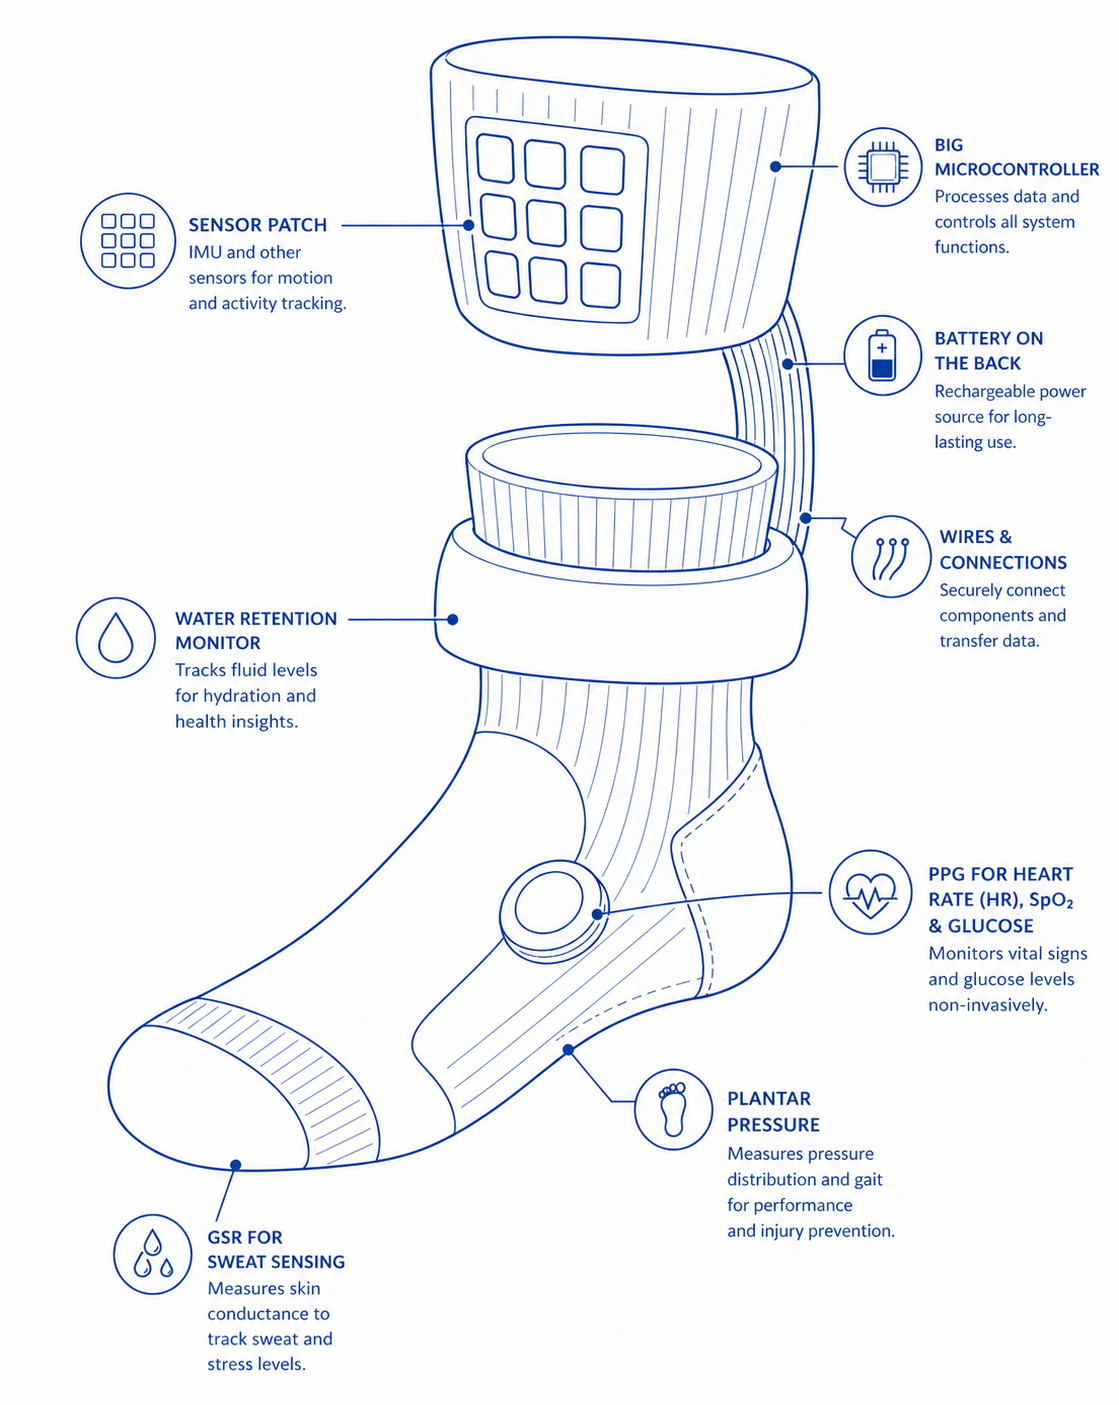
\includegraphics[width=0.65\textwidth]{FYP_Template_Spring/Figures/L.png}
        \caption{Initial Design of Alternative 2}
        \label{fig:L}
    \end{figure}

\subsection{Design Alternative 3: Wearable Sock}
To improve patient compliance and increase device wear time, this design alternative (Fig.~\ref{fig:Sock}) reduces the number of sensors employed. Given the need for both continuous monitoring and user comfort, the selected parameters were carefully chosen, and any sensing modalities not relevant to neurodegenerative disease monitoring were excluded. The selected parameters are as follows:
\begin{itemize}
    \item Plantar Pressure
    \item SpO$_2$
    \item Heart Rate
    \item Water Retention
\end{itemize}

However, this design is limited to indoor use. Since a shoe cannot be worn over the sock, patients with active or busy lifestyles would experience a significant reduction in device wear time. Consequently, Design Alternative 4 was considered.\\

\begin{figure}[H]
    \centering
    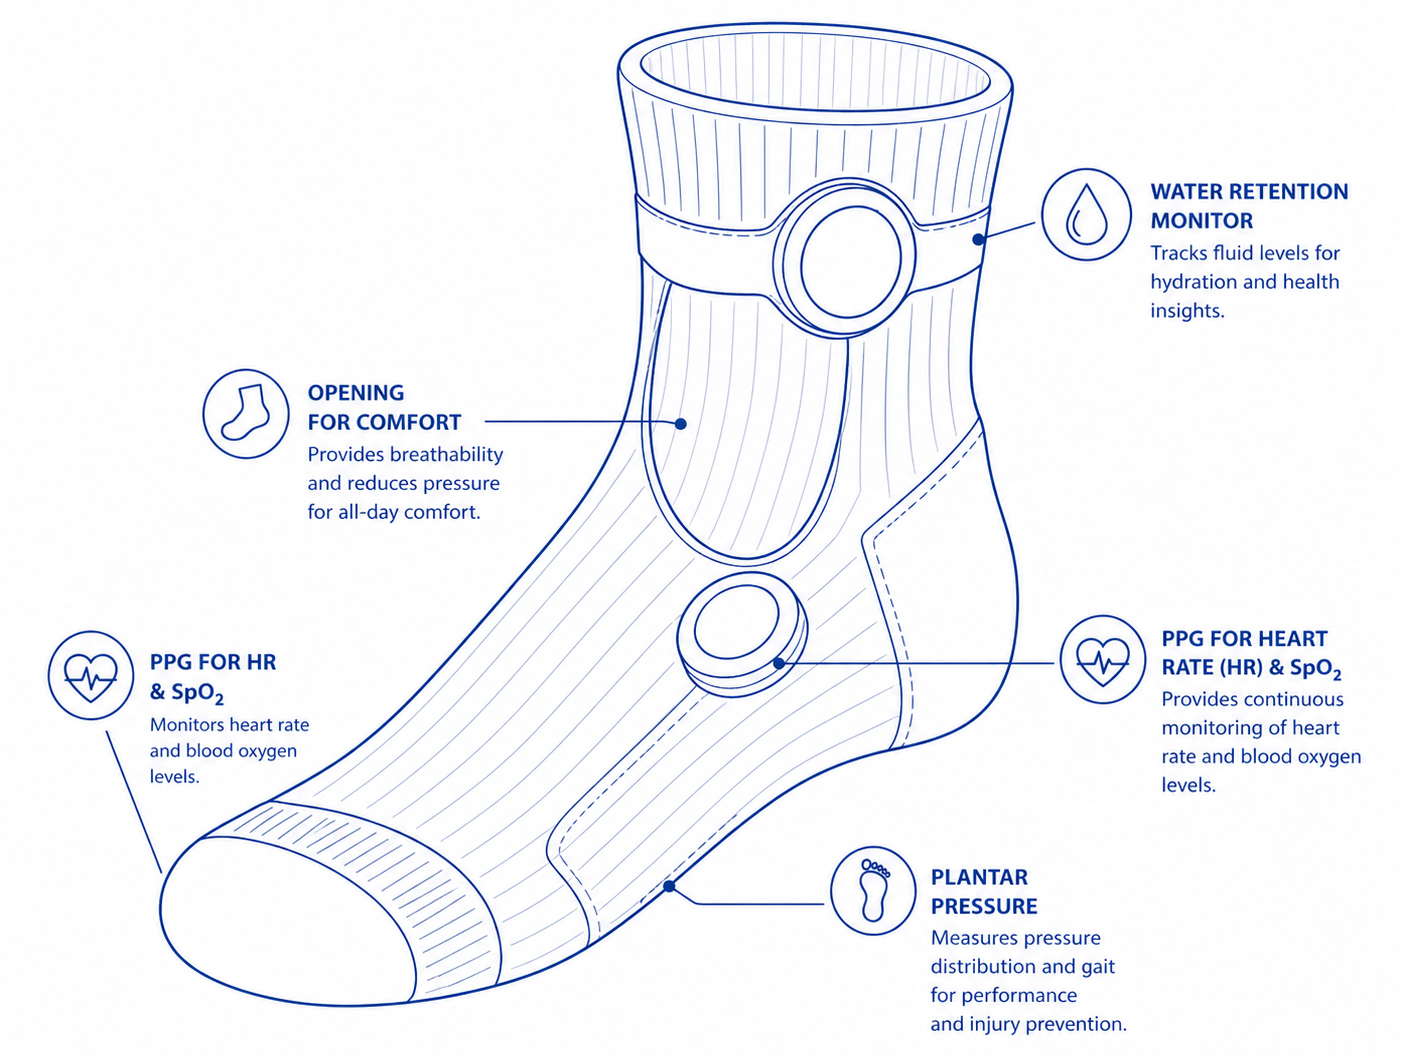
\includegraphics[width=0.65\textwidth]{FYP_Template_Spring/Figures/sock.png}
    \caption{Initial Design of Alternative 3}
    \label{fig:Sock}
\end{figure}

%\noindent Then, the sensors' location were chosen very carefully. Since cardiovascular disease may cause water retention in the foot and ankle, it was agreed that the heart rate and SpO$_2$ sensor are to be placed in two locations. This redundancy will be used to minimize errors related to water retention. This enables cross-checking the readings and reducing the impact of water retention-related noise or even sensor failure.
  
\subsection{Final Design: The Sandals}
To overcome the limitations of the previous design alternatives, a sandal-based wearable was proposed, as shown in Fig. ~\ref{fig:Sandals}. This design enables continuous monitoring in real-world environments, both indoor and outdoor, without restrictions. Unlike the sock, the sandals can be comfortably worn for extended periods of time in different scenarios and situations, which increases patient compliance and user wear time.\\   

The open and structured design allows for direct contact with the sensors, which in turn, allows for more robust sensor readings. The selected sensing modalities can be embedded in the straps of the sandals. This configuration enhances the real-world durability by protecting the components from various environmental factors, making it suitable for long-term monitoring applications.

\begin{figure}[H]
    \centering
    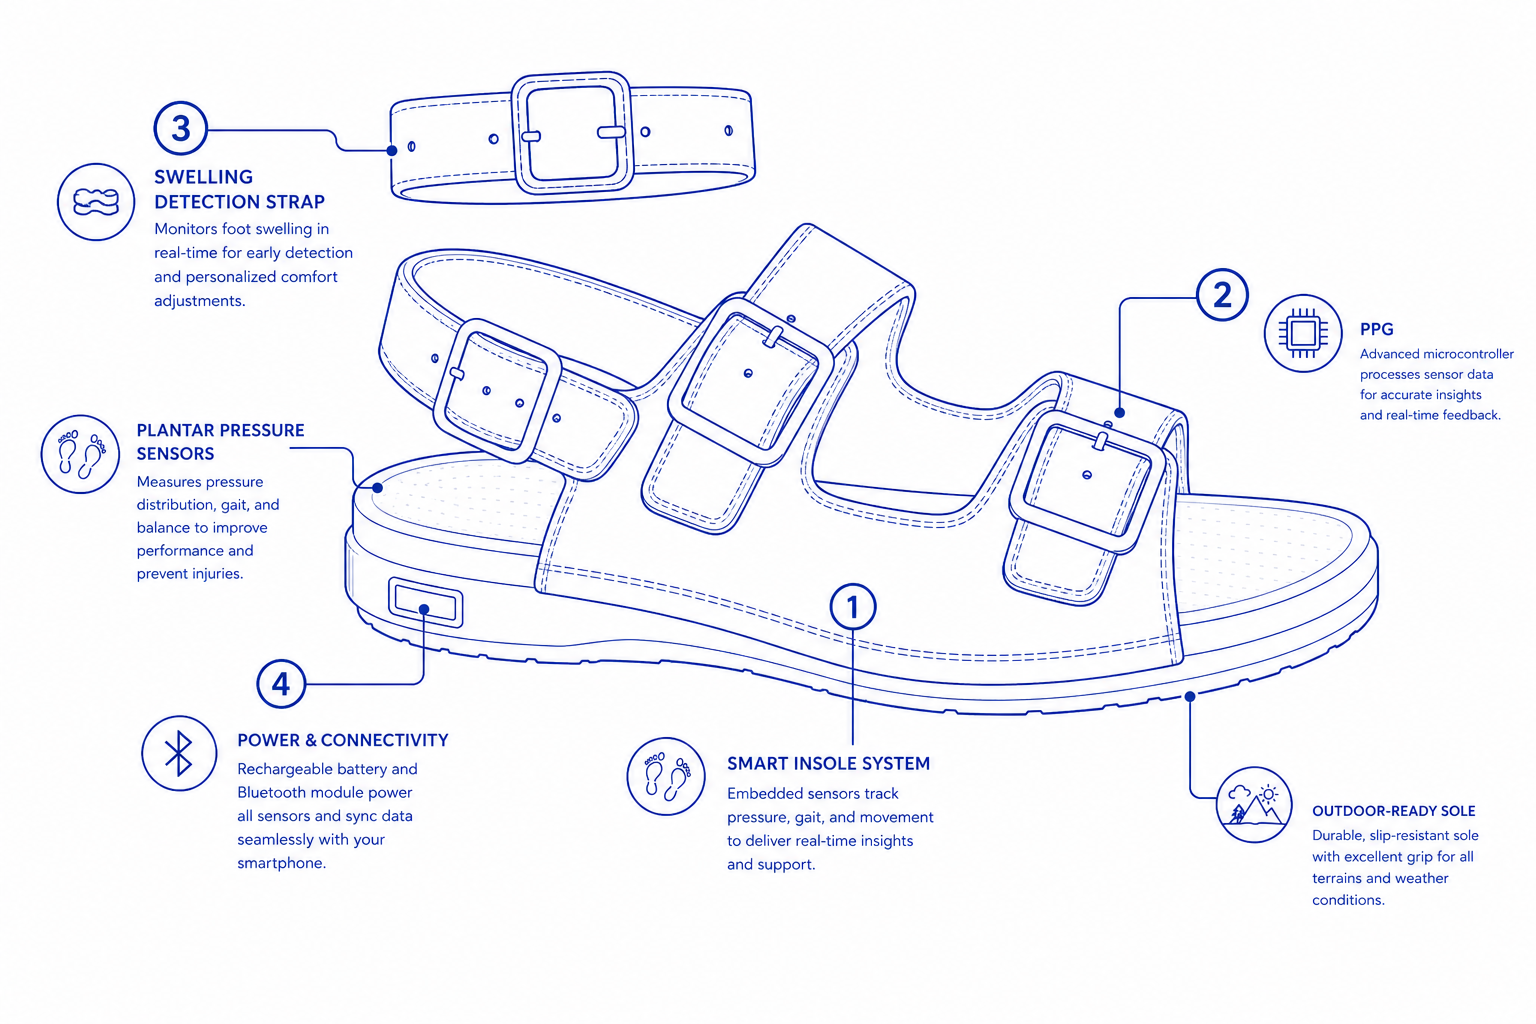
\includegraphics[width=0.75\textwidth]{FYP_Template_Spring/Figures/sandals.png}
    \caption{Initial Design of the Chosen Design.}
    \label{fig:Sandals}
\end{figure}

The evaluation and comparison of design alternatives, as seen in Table ~\ref{tab:CDA}, dictates the clear winner: \textbf{Final Design:} \textit{The Sandals} seen in Fig. ~\ref{fig:Sandals}. This is mainly due to its clinical relevance, patients' comfort, scalability and expandability, and wearability and real-world durability. \\

\begin{table}[H]
\centering
\footnotesize
\caption{Comparison of Design Alternatives}
\label{tab:CDA}
\renewcommand{\arraystretch}{1.2}

\begin{adjustbox}{center,max width=\textwidth}
\begin{tabular}{p{2.5cm}p{2.5cm}p{2.5cm}p{2.5cm}p{2.5cm}p{1.5cm}}
\hline
\textbf{Criteria} & \textbf{Clinical Mat} & \textbf{Wearable L} & \textbf{Wearable Sock} &
\textbf{Sandals} &
\textbf{Total} \\ \hline
Clinical Relevance & 6 & 9 & 18 & 18 & 18 \\
Patient Comfort & 17 & 4 & 15 & 17 & 17 \\
Wearability \& Real-World Durability & 2 & 6 & 8 & 9 & 10 \\
Practical Feasibility & 10 & 5 & 8 & 9 & 10 \\
Cost \& Component Availability & 10 & 5 & 9 & 9 & 10 \\
Data Quality/Robustness & 17 & 9 & 15 & 16 & 18 \\
Ease of Calibration \& Maintenance & 6 & 4 & 5 & 4 & 7 \\
Scalability \& Expandability & 3 & 5 & 9 & 8 & 10 \\
\hline
\textbf{Overall Grade} & \textbf{71} & \textbf{47} & \textbf{87} & \textbf{90} & \textbf{100} \\
\hline
\end{tabular}
\end{adjustbox}

\end{table}

\section{Design Decisions} 
%All design decisions must be related to the outlined constraints and specifications.\\
Based on the comparison of the proposed design alternatives, the final design decision was to proceed with the sandal-based wearable system. This decision was not only based on the numerical score shown in Table~\ref{tab:CDA}, but also on the practicality of using the device in real-life conditions. From the beginning of the project, the main aim was not simply to create a sensing system that works in a controlled environment, but to develop a device that a patient would be willing to wear for a long period of time without feeling restricted. For this reason, patient comfort, wearability, durability, sensing reliability, and ease of use were treated as major factors in the final decision. \\

The clinical mat was initially considered because it provides a controlled way of capturing plantar pressure data. However, this design remained limited to clinical or laboratory settings requiring frequent clinical visits. Since ataxia-related changes may appear gradually and may not always be captured during occasional clinical visits, this alternative did not fully satisfy the need for continuous monitoring. The decision was therefore made to move away from a stationary system and toward a wearable design that collects data while the patient applies his/her daily routine. \\


\noindent This introduced the need for a design similar to the wearable L design which serves the purpose of monitoring several physiological and biomechanical parameters from the foot. Although this alternative was clinically rich, it was also too bulky and complex for daily use. Including many sensors would increase the wiring complexity, power consumption, calibration effort, and cost of the prototype. More importantly, it could reduce patient compliance, since a device that feels heavy or uncomfortable is less likely to be worn consistently. Therefore, the design was simplified by keeping only the sensing modalities that directly support the project objectives. \\

The wearable sock was then considered as a more comfortable and less bulky alternative. This design helped narrow the sensing parameters to plantar pressure, SpO$_2$, heart rate, and water retention. However, the sock introduced another practical limitation which is that it is mainly suitable for indoor use only. Since patients can not comfortably wear regular shoes over a  sock filled or wrapped with sensors, the expected wear time would decrease, especially for users with active daily routines. This limitation affected the real-world usability of the system and motivated the transfomation into a sandal-based design. \\

Accordingly, the sandal design was selected as the final design direction. The sandal structure provides a better balance between sensing performance and user comfort and daily usability. It allows the plantar-pressure sensors to remain in direct contact with the sole of the foot, while the straps provide suitable locations for integrating the additional sensing components. This makes the system less restrictive than a sock and more realistic than a clinical mat. The open structure also improves accessibility during testing, maintenance, cleaning and calibration, since the sensors and electronic connections can be inspected and adjusted more easily. Another major decision was to focus the system on a reduced set of sensing parameters. Plantar pressure was kept as the core sensing modality because it is directly related to gait and balance changes, which are important indicators for ataxia monitoring. Heart rate and SpO$_2$ were included because they provide additional physiological context through the PPG sensor. Swelling was also included because swelling in the foot or ankle may affect both patient comfort and sensor readings. \\ %Other sensing ideas, such as non-invasive glucose sensing and sweat analysis, were excluded at this stage because they would increase complexity without directly supporting the main project objective. \\

 For the plantar-pressure subsystem, the design decision was to use a matrix-based sensing structure rather than isolated pressure points. This allows the system to reconstruct pressure distribution across the foot instead of only measuring force at a few separate locations or just choosing few important points whose number is limited to the microcontroller's analog pins. The matrix structure supports the generation of pressure maps or heatmaps, which are more useful for observing gait-related changes and are later fed as inputs to the machine-learning model for ataxia detection. To reduce the number of required microcontroller pins, multiplexers were used to scan the sensing matrix. This decision helped keep the system more compact and feasible while still maintaining the ability to collect spatial pressure information. \\

The placement of the sensors was also decided based on both technical and usability constraints. The pressure-sensing layer was placed under the foot to capture plantar loading during standing and walking. The PPG sensor was positioned in a strap location that allows contact with the skin, especially the toes where veins are somehow visible, while reducing interference from excessive movement. The swelling-detection sensors were placed around the ankle region, where changes in circumference can be observed more clearly. These placements were chosen to improve signal quality without making the device uncomfortable or difficult to wear. \\

The final design also considered power, communication, and integration constraints. Since the device is intended to operate as a wearable system, the electronics had to remain compact and low-power. Wireless communication was selected to allow the collected data to be transmitted to the mobile application without restricting the user's movement. This supports the overall goal of continuous monitoring, since the patient does not need to stay connected to a computer or clinical workstation during use. \\

Another design decision was related to the protection of the electronic components and the overall durability of the prototype. Since the device is still in the prototype stage, a final certified IP rating was not assigned. However, environmental protection was still considered during the design process, especially because the sandal is intended for real-world use where it may be exposed to dust, light splashes, water, moisture and other outdoor conditions. After mounting and integrating the sensors on the sandal, the decision was made to cover the external electronic areas using an added leather layer. This layer acts as a protective barrier and improves the overall appearance of the prototype hiding all complex wiring scenes, while also reducing direct exposure of the sensors. Instead of permanently sewing the leather from all sides, Velcro was selected for part of the attachment. This allows the cover to be opened when needed for troubleshooting, sensor adjustment, wiring inspection, or maintenance. Although a fully sealed design would be more suitable for a finalized product, the use of removable leather covering was more practical for the current prototype because it balances protection with accessibility. In future iterations, once the internal layout is finalized and no frequent modifications are needed, the covering can be made more permanent and properly sealed to support a clearer water-resistance target and a possible IP rating. \\

Overall, the final sandal-based design was selected because it provides the best compromise between clinical relevance, patient comfort, technical feasibility, and real-world durability. It keeps the essential sensing functions needed for the project while avoiding unnecessary complexity. The sandal structure also supports the integration of protective covering around the electronic components, which helps improve durability while keeping the prototype accessible for troubleshooting and maintenance. This design direction leaves room for future improvements, since additional sensors, updated modules, or a more permanent sealed enclosure can be integrated into the sandal structure without changing the overall concept of the system. \\

\section{Design Iterations} 

% \textbf{It is highly encouraged to utilize diagrams and illustrations.} 


\subsection{Refinement of the Sensing Scope}
\label{subsec:iteration_sensing_scope}

%ADD A Visual

\noindent The first iteration involved narrowing the sensing scope from a broad multi-sensor concept to a focused set of clinically relevant parameters. Early ideas included plantar pressure, heart rate, SpO$_2$, swelling detection, non-invasive glucose sensing, sweat analysis, and general motion tracking. However, including all of these modalities would have increased wiring complexity, power consumption, calibration effort, and cost. \\

\noindent The design was therefore refined to focus on plantar pressure, PPG-based cardiovascular monitoring, and swelling detection. This reduced the complexity of the prototype while preserving the main project objectives which are gait monitoring, cardiovascular assessment, and ankle/foot swelling support. \\



\subsection{Plantar-Pressure Matrix Refinement}
\label{subsec:iteration_pressure_matrix}

\noindent The plantar-pressure subsystem went through several circuit iterations before reaching the final Velostat-based matrix configuration. The first stage was a simple proof-of-concept using a single force-sensitive resistor (FSR), shown in Fig.~\ref{fig:single_fsr_iteration}. This test was used to verify the basic pressure-sensing principle and confirm that an applied force could be converted into a measurable analog voltage.

\begin{figure}[H]
    \centering
    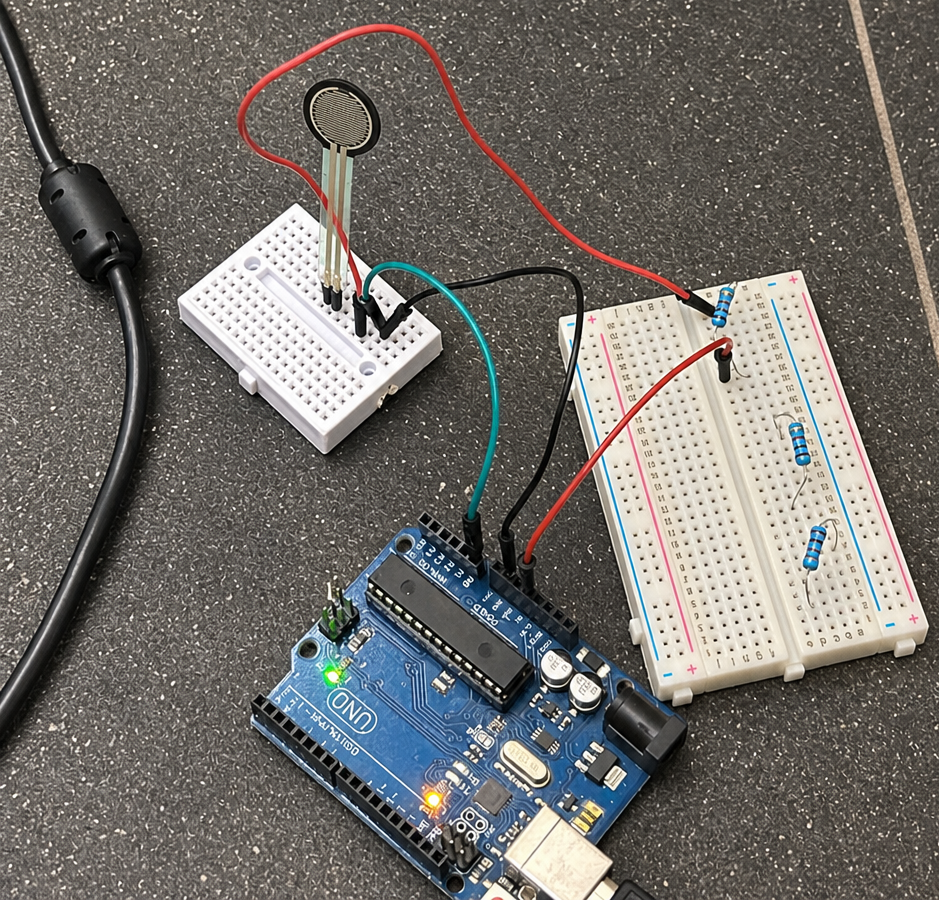
\includegraphics[width=0.65\textwidth]{FYP_Template_Spring/Figures/pressure with 1 FSR.png}
    \caption{Initial pressure-sensing proof-of-concept using a single FSR.}
    \label{fig:single_fsr_iteration}
\end{figure}

\noindent After validating the single-sensor circuit, the setup was expanded to three FSRs, as shown in Fig.~\ref{fig:three_fsr_iteration}. This iteration was used to test whether multiple pressure readings could be collected simultaneously and arranged into a small pressure map. It helped the team explore the possibility of generating a basic heatmap from discrete pressure sensors before moving toward a larger plantar-pressure sensing surface.

\begin{figure}[H]
    \centering
    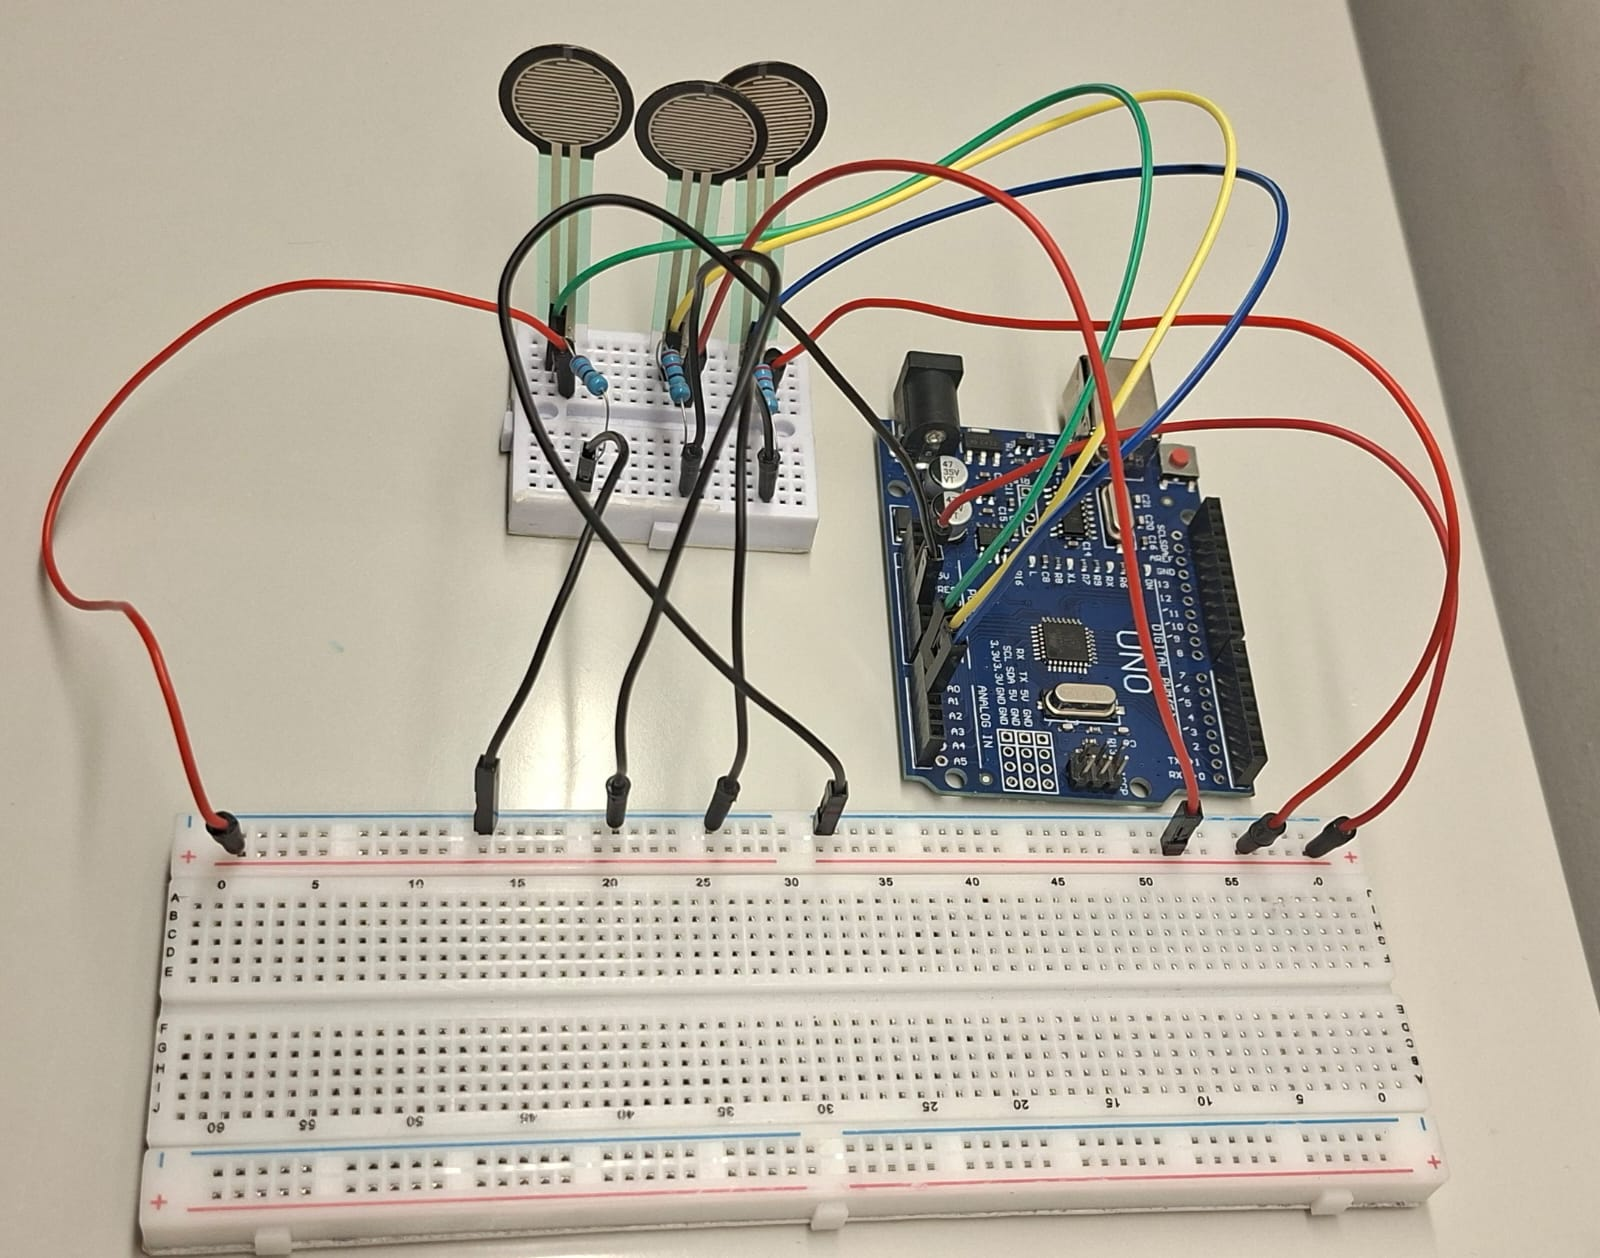
\includegraphics[width=0.75\textwidth]{FYP_Template_Spring/Figures/3FSRs.jpeg}
    \caption{Three-FSR prototype used as an intermediate multi-point pressure-sensing test.}
    \label{fig:three_fsr_iteration}
\end{figure}

\noindent However, the FSR-based approach revealed several limitations. The sensors saturated quickly under applied load, which reduced their ability to distinguish between different pressure levels. In addition, using FSRs to capture a meaningful plantar-pressure distribution would require a large number of individual sensors placed across the foot. This would increase cost, wiring complexity, calibration effort, and the number of required analog inputs. This was not practical with the selected microcontroller, since the Arduino provides a limited number of available analog and digital pins, and connecting each FSR individually would quickly exceed the available pin count. Other alternatives, such as load cells or rigid pressure sensors, were also not suitable because they are bulky, expensive, and difficult to integrate into a wearable device intended for standing and walking.\\


\noindent These limitations motivated the transition from isolated pressure sensors to a Velostat-based pressure matrix. Instead of using many separate pressure sensors, the Velostat design allowed the team to create a larger sensing surface using conductive traces and a pressure-sensitive layer. This made the system more suitable for plantar-pressure mapping while keeping the sensing layer flexible enough for integration into the wearable prototype. \\


\noindent The next design iteration introduced a three-multiplexer configuration, shown in Fig.~\ref{fig:three_mux_iteration}. This stage marked the transition from discrete pressure sensing to a matrix-based scanning approach. Multiplexers were introduced to reduce the number of required microcontroller pins while allowing a larger number of sensing points to be scanned.

\begin{figure}[H]
    \centering
    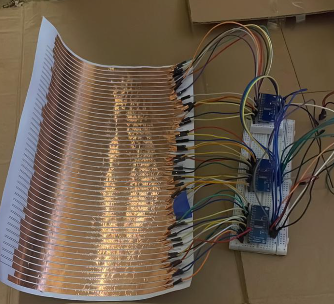
\includegraphics[width=0.75\textwidth]{FYP_Template_Spring/Figures/3_mux_config.png}
    \caption{Intermediate three-multiplexer configuration used during plantar-pressure matrix development.}
    \label{fig:three_mux_iteration}
\end{figure}

\noindent After testing the three-multiplexer setup, the readout electronics were consolidated into the
\textbf{final muxed matrix circuit} shown in Fig.~\ref{fig:four_mux_iteration}, which matches the
configuration implemented today in the Arduino firmware (\texttt{pressure\_reader.h/.cpp}). The
Velostat-based sensing surface is organised as a \textbf{$43 \times 14$} grid (602 active sites).
Electrical addressing is \emph{not} one sensor per MCU pin; instead, the matrix is wired as a
classical row--column scan with analogue readout. \\

\noindent \textbf{Row drive (three multiplexers, one shared address bus).} Four digital select lines
\texttt{S0--S3} (Arduino pins D2--D5) drive three separate 16-channel row multiplexers in parallel.
Each multiplexer has its own output-enable / strobe line: \texttt{SIG1} on D10, \texttt{SIG2} on
D11, and \texttt{SIG3} on D12. The firmware asserts \emph{at most one} of \texttt{SIG1--SIG3} at a
time so that only one row driver IC is electrically tied into the row bus, while the other two are
held inactive. For a given logical row index, the firmware maps that index to a specific 4-bit
channel code on \texttt{S0--S3} and then raises the appropriate \texttt{SIG*} line, inserting a
short settling delay (\SI{20}{\micro\second}) before any column sampling occurs. Some physical
multiplexer channels at the ends of each bank are intentionally unused so that the electrical mesh
matches the intended PHBLE footprint without scanning empty interconnect. \\

\noindent \textbf{Column read (one analogue multiplexer, single ADC).} All column lines are routed
through a fourth 16-channel multiplexer whose select lines are also four bits wide, wired to D6--D9.
The multiplexer output is connected to a \emph{single} analogue input, \textbf{A0}, where the
Nano~33~BLE's ADC samples each intersection at \textbf{12-bit} resolution (values are masked to
12~bits in software). Column addressing likewise skips the outermost mux channels that are not
bonded out to the 14 active columns. After each column address change, the firmware waits
\SI{20}{\micro\second} before sampling the selected column on \texttt{A0} so that the mux and the resistive node
can settle. \\

\noindent \textbf{Scanning outcome.} One complete frame therefore consists of 43 successive row
selections, each followed by 14 ADC conversions---all realised with only \textbf{one} dedicated
analogue pin for the entire matrix, plus the shared digital address and enable pins described
above. This is the circuit that feeds the pressure-reading path in the deployed application. \\

\begin{figure}[H]
    \centering
    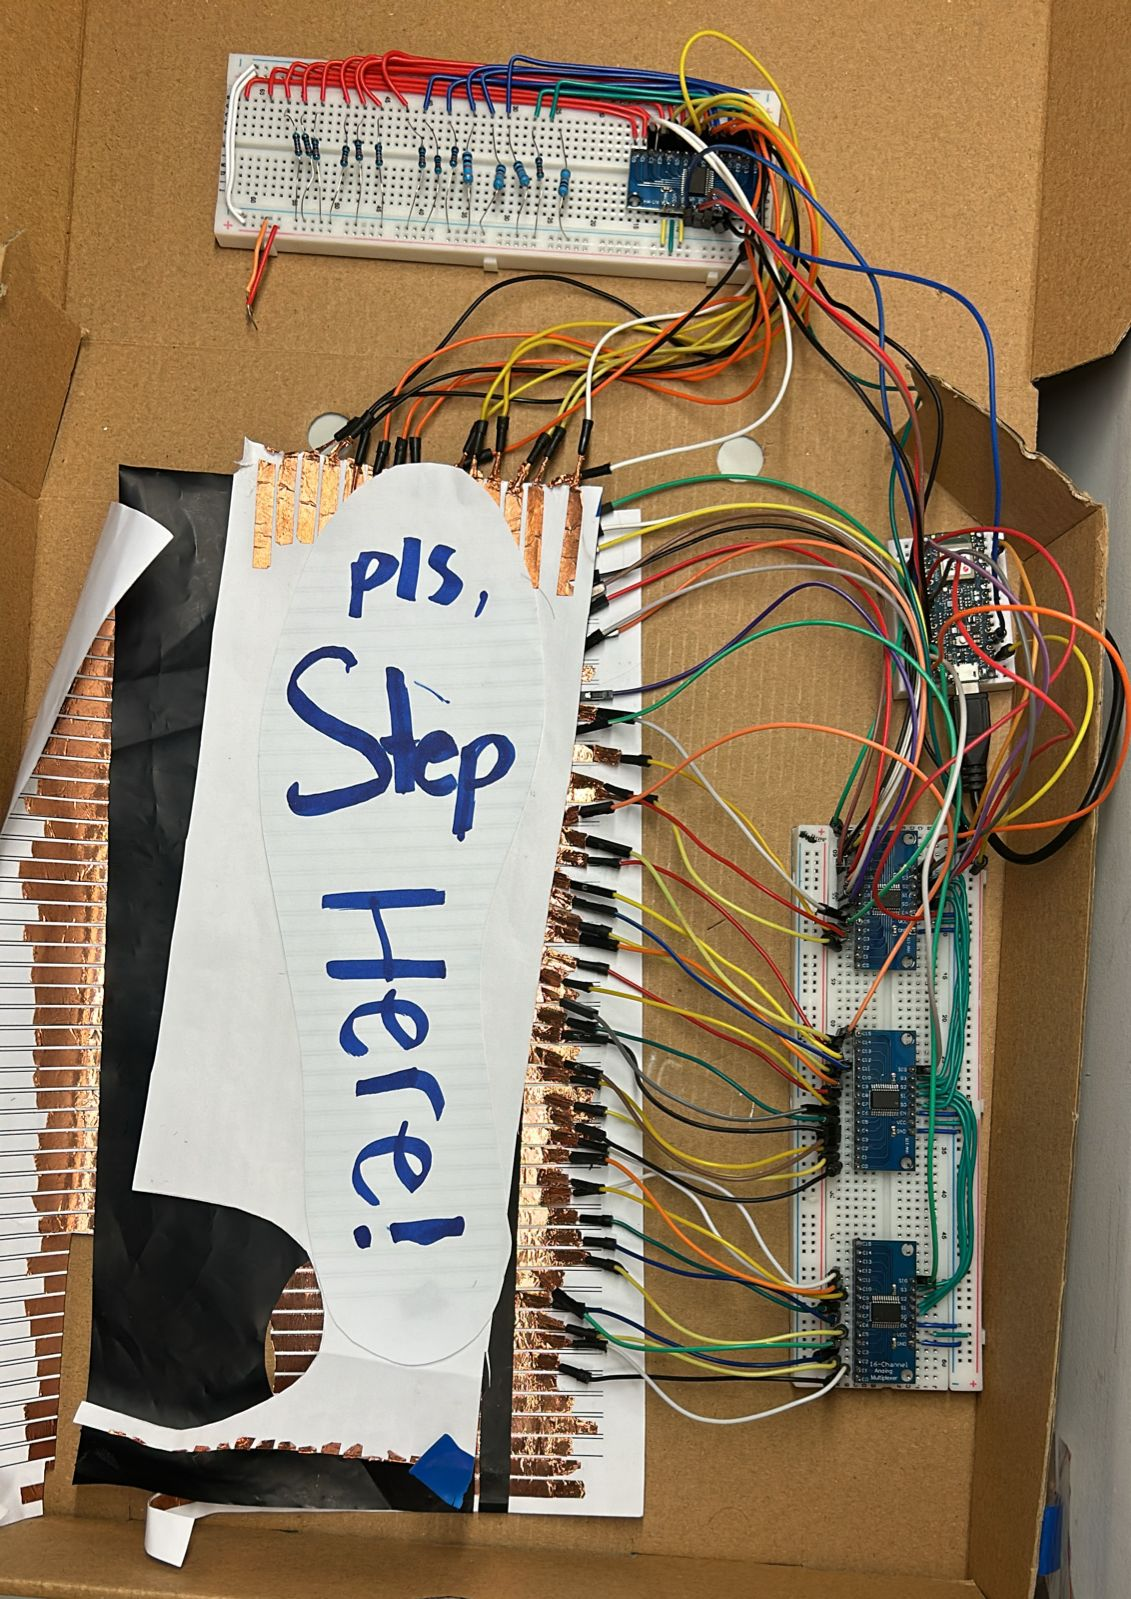
\includegraphics[width=0.75\textwidth]{FYP_Template_Spring/Figures/velo_final_circuit.jpeg}
    \caption{Final Velostat matrix readout: three row-driving multiplexers (shared \texttt{S0--S3},
             separate \texttt{SIG1--SIG3}) plus one analogue column multiplexer into \texttt{A0}.}
    \label{fig:four_mux_iteration}
\end{figure}

\noindent Overall, this design iteration moved from discrete FSR experiments to a muxed Velostat
matrix whose \textbf{documented electrical interface} (four multiplexers, single ADC, $43 \times 14$
sites) is the one now implemented in firmware for plantar-pressure acquisition. \\




\subsection{Swelling Detection Refinement}
\label{subsec:iteration_swelling_detection}

\noindent The swelling-detection subsystem went through several iterations before reaching the final configuration. The initial approach used two flex sensors mounted on a Velcro strap around the ankle. This setup was intended to detect swelling through changes in sensor bending and raw deviation values. However, early testing made it clear that the Velcro strap was too rigid and did not deform consistently or expand with changes in circumference. As a result, the flex sensors did not always respond reliably to simulated swelling conditions. \\

\noindent To test the concept further, swelling was initially simulated by inserting an expandable object under the strap. However, this did not accurately represent the gradual and distributed circumference change expected in real ankle swelling. The tightness and stiffness of the Velcro also affected the readings, making it difficult to distinguish between actual circumference change, strap pressure, and sensor repositioning. This showed that the sensing mechanism needed to be less dependent on local pressure at one point and more representative of the overall ankle geometry. \\

\noindent A second approach was then explored using a more belt-like or stretchable support to improve contact between the flex sensors and the ankle surface. Although this improved adjustability compared to the original Velcro setup, the two-sensor configuration still provided limited information because it measured only a combined deviation rather than estimating the shape or size of the monitored ankle region. This made the output sensitive to sensor placement and difficult to relate to a physical swelling measurement. \\

\noindent Based on these limitations, the swelling subsystem was refined into a four-sensor, dual-level configuration. Instead of relying only on raw deviation from two sensors, the updated approach allowed the system to estimate upper and lower circumference changes and use them to represent the monitored ankle segment more realistically. The detailed calibration method and volume-estimation model are discussed later in the implementation section, while this iteration highlights the design transition from a simple deviation-based idea to a more physically meaningful swelling-estimation approach. \\








\subsection{PPG Placement and Signal Acquisition}
\label{subsec:iteration_ppg_signal}

\subsubsection{Sensor placement on the wearable}

\noindent Photoplethysmography on a foot-worn device is inherently more challenging than on a fingertip
or wrist, because perfusion is weaker and motion artefacts are stronger during ambulation. The
integrated prototype therefore mounts the MAX30102 module on a sandal strap where it can press
gently against the skin of the forefoot and toe region, chosen as a compromise between optical
coupling (enough pulsatile blood volume for red and infrared channels) and mechanical stability.
The strap tension was tuned so that the LEDs maintain contact without creating pressure so high
that it collapses the local microvasculature. This placement keeps the cardiovascular sensor on the
same wearable as plantar pressure and swelling-related sensing, at the cost of requiring more
aggressive acquisition and validation in software than would be needed for a classic finger clip. \\

\subsubsection{Acquisition chain and processing pathways}

\noindent The MAX30102 is driven over the microcontroller's I\textsuperscript{2}C bus and read through
its internal FIFO, which delivers paired red and infrared photodiode samples produced by the
integrated LED drivers. The front end is configured so that samples are not averaged in the FIFO
before read-out, preserving the full temporal structure of the pulsatile waveforms. On every pass of
the main firmware loop the driver may pull several FIFO entries in one batch so that brief stalls
from other subsystems (for example Bluetooth or the pressure matrix) do not leave the FIFO to
overflow; those samples fill a fixed-length analysis window. Once that window is complete, a batch
estimator updates heart rate and SpO\textsubscript{2} jointly from the same segment. \\

\noindent \textbf{Purpose of the heart-rate and SpO\textsubscript{2} algorithm.} Foot-worn PPG is
easily contaminated by motion, pressure changes at the skin interface, and intermittent loss of
contact. A practical estimator must therefore (i)~\emph{reject} segments where the two colour
channels no longer describe the same underlying cardiac pulsation, and (ii)~\emph{stabilise} rate
estimation against narrow impulsive spikes that confuse simple peak counting. The implemented
approach addresses (i) by requiring strong agreement between the red and infrared traces after
detrending, and (ii) by inferring the pulse period from the autocorrelation structure of the infrared
waveform rather than from isolated maxima alone. SpO\textsubscript{2} is only computed once a
reliable period has been found, using a classical ratio-of-ratios style construction so that
saturation estimates track the relative pulsatile strengths of the two wavelengths. The wearable
only forwards a new HR/SpO\textsubscript{2} pair to the application when \emph{both} quantities pass
their validity checks for the same window, so that a marginal SpO\textsubscript{2} value is never
shown without a consistent heart-rate estimate. \\

\noindent \textbf{Mathematical structure.} Let $\{x_k\}_{k=0}^{N-1}$ and $\{y_k\}_{k=0}^{N-1}$ denote
the raw infrared and red sample counts in one window. Each channel is mean-centred,
$\tilde{x}_k = x_k - \bar{x}$ and $\tilde{y}_k = y_k - \bar{y}$ with $\bar{x}=\frac{1}{N}\sum_k x_k$
(and analogously $\bar{y}$). A shared discrete time index $t_k = k - \frac{N-1}{2}$ removes slow
linear drift by subtracting a least-squares slope from each centred channel,
\begin{equation}
  x^{\dagger}_k = \tilde{x}_k - \beta_x\, t_k, \qquad
  y^{\dagger}_k = \tilde{y}_k - \beta_y\, t_k,
\end{equation}
where $\beta_x$ (respectively $\beta_y$) minimises $\sum_k (\tilde{x}_k - \beta_x t_k)^2$ (and the
red analogue). After this step the waveforms are dominated by the pulsatile AC component. Let the
root-mean-square (AC) amplitudes be
\begin{equation}
  A_x = \sqrt{\frac{1}{N}\sum_{k=0}^{N-1} \bigl(x^{\dagger}_k\bigr)^2}, \qquad
  A_y = \sqrt{\frac{1}{N}\sum_{k=0}^{N-1} \bigl(y^{\dagger}_k\bigr)^2}.
\end{equation}
Agreement between the two colour channels is quantified by the Pearson correlation coefficient
\begin{equation}
  \rho_{x,y} =
  \frac{\frac{1}{N}\sum_{k=0}^{N-1} x^{\dagger}_k\, y^{\dagger}_k}{A_x\, A_y},
\end{equation}
which must exceed a high threshold (in firmware, $\rho_{x,y}\ge 0.8$) before the segment is accepted
for further processing. If this gate fails, the window is discarded for both metrics. \\

\noindent For accepted windows, the infrared residual $\{x^{\dagger}_k\}$ is analysed in the lag
domain. The (biased) autocorrelation at integer lag $L$ is
\begin{equation}
  R(L) = \frac{1}{N-L}\sum_{k=0}^{N-L-1} x^{\dagger}_k\, x^{\dagger}_{k+L}, \qquad 0 < L < N,
\end{equation}
and a search restricted to lags compatible with a plausible resting-to-exercise heart-rate band
selects a refined lag $L^\star$ that characterises one cardiac cycle. Writing $\tau$ for the
beat-to-beat interval implied by that lag under the acquisition chain's uniform sampling cadence,
heart rate in beats per minute is
\begin{equation}
  \mathrm{HR} = \frac{60}{\tau}.
\end{equation}
Algorithmically, $\tau$ is inferred from $L^\star$ and the structured maxima of $R(L)$, so that
$\mathrm{HR}$ tracks the dominant periodicity of the detrended infrared waveform rather than
isolated amplitude spikes. \\

\noindent Given a valid $L^\star$, SpO\textsubscript{2} is derived from a ratio that couples AC and
DC information from both wavelengths,
\begin{equation}
  R_{\mathrm{oxy}} = \frac{A_y\,\bar{x}}{A_x\,\bar{y}},
\end{equation}
where $\bar{x}$ and $\bar{y}$ are the original window means (DC levels). When
$0.02 < R_{\mathrm{oxy}} < 1.84$, the saturation estimate is evaluated with the empirical cubic
calibration
\begin{equation}
  \mathrm{SpO}_2 =
  \bigl(-45.060\, R_{\mathrm{oxy}} + 30.354\bigr)\, R_{\mathrm{oxy}} + 94.845
  \quad (\%).
\end{equation}
Values of $R_{\mathrm{oxy}}$ outside the admissible interval invalidate SpO\textsubscript{2} for
that window. Overall, correlation gating enforces dual-wavelength consistency, autocorrelation-based
period estimation stabilises HR on short windows, and the polynomial maps a physically motivated
ratio to a percentage oxygen saturation only when the entire chain of checks succeeds. If heart rate
or SpO\textsubscript{2} fails at any stage, the firmware withholds both from the host until a later
window passes every test. \\

\noindent \textbf{625-sample waveform at 125~Hz.} Separately from the batch HR/SpO\textsubscript{2}
path above, the system supports a \textbf{five-second} photoplethysmography trace formatted as \textbf{625 samples at
an effective 125~Hz}, aligned with the blood-pressure estimation model on the mobile side. Achieving
that rate does not rely on the main loop running exactly every eight milliseconds; instead, during
scheduled short acquisition intervals the optical front end is temporarily switched to a higher
internal sample rate so the FIFO always contains fresh IR data. A software timer keyed on elapsed
microseconds then decides when each output sample is due: at each 125~Hz tick the firmware takes the
\emph{most recent} IR value available (non-blocking FIFO drain), applies light exponential smoothing
and a consistent sign convention so peaks appear in a stable orientation, and appends the value to a
625-sample buffer. Once the buffer is complete it represents exactly five seconds of uniformly spaced
waveform data at 125~Hz and can be transmitted wirelessly in segments for reconstruction on the phone.
Outside those intervals the front end returns to the lower-rate configuration used for routine heart
rate and SpO\textsubscript{2} updates, so the higher-rate path is reserved for waveform quality rather
than running continuously at maximum LED duty. \\

\subsection{Power Stabilization and Hardware Compactness}
\label{subsec:iteration_power_hardware}

\noindent The power-supply design also went through multiple iterations because the prototype had to be both electrically stable and physically compact enough to fit on the wearable. The initial plan was to use a single 3.7~V Li-Po battery connected to a TP4056 charging module, followed by a compact DC-DC step-up converter to provide a regulated 5~V supply for the Arduino. This configuration was preferred because it used only one battery cell and could keep the wearable lighter and less bulky. However, the required compact step-up converter was not available during the development period, which delayed this design direction. \\

\noindent As an alternative, the team considered using two 3.7~V Li-Po batteries in series and stepping the voltage down to 5~V using a DC--DC step-down converter. Although this approach could provide the required voltage level, it introduced additional bulk and increased the complexity of the power system. A two-cell configuration would also require more careful charging and protection circuitry, making it less suitable for a compact foot-worn prototype. For this reason, this option was rejected despite being electrically feasible. \\

\noindent The final iteration returned to the single-cell Li-Po configuration. The battery was connected to the TP4056 charging module, and a smaller available step-up converter was used to raise the battery voltage to the regulated level required by the Arduino and the sensing electronics. This solution provided a better balance between voltage stability, component availability, and wearable compactness. It also reduced the physical size of the power system compared to the two-battery alternative, making it more practical for integration into the sandal-based prototype. \\







\subsection{Data Encryption}
\label{subsec:iteration_enc}










\section{Standards}
%You need to include the list of all the applicable standards to your project and how they are related to the decisions made during the design process. Make sure to include citations for all standards used (IEEE, ITU, etc…). \\
%\newline
%The IEEE standards can be found on link: \href{https://standards.ieee.org//}{[IEEE Standards]}

In engineering design, especially for biomedical and embedded systems, following the internationally recognized standards is a must if safety, reliability, and interoperability are to be guaranteed. The standards that apply set the accepted frameworks, testing procedures, and performance requirements that the engineering solutions will have to go through during the design, implementation, and validation phases. Because of the electronic hardware, biomedical sensing, wireless communication, and data transmission that this project comprises, it will have to comply with several existing regulations that control these areas.\\

\vspace{0.05cm}

\noindent This project is based on \textbf{IEEE (Institute of Electrical and Electronics Engineers)} norms for the creation of our foot-wearable biomedical gadget. IEEE standards are regarded as the basis of world technology growth, establishing the foundation for communication protocols, software quality, and medical device interoperability \cite{IEEEStandards2025}. The next subsections introduce every standard in detail, illustrating its definition, principal aim, and direct relation to our proposed solution.\\

\subsection{Definition and Purpose of Relevant Standards}

\begin{itemize}
    \item \textbf{IEEE 802.15.1 – Wireless Personal Area Networks (Bluetooth) \cite{ieee802151}}  
    It establishes close-range, low-energy wireless communication protocols that are the foundation of Bluetooth technology. It also provides secure, efficient, and interoperable data transfer among devices in a personal area network.

    \item \textbf{IEEE 802.15.6 – Wireless Body Area Networks (BAN) \cite{ieee802156}}  
    It requires that wireless communication be minimal energy-consuming for gadgets that are placed on, inside, or near the human body. It also guarantees secure and reliable data transfer for devices that are wearable or used in the field of medicine.

    \item \textbf{IEEE 11073 – Health Informatics and Medical Device Communication \cite{ieee11073}}  
    It defines the standards for medical device interoperability and health informatics communication. This enables precise and standardized data exchange between medical sensors, devices, and health care systems.

    \item \textbf{IEEE 1451 – Smart Transducer Interface for Sensors and Actuators \cite{ieee1451}}  
    It defines standard procedures for intelligent sensors and actuators, which cover calibration, data formats, and metadata structures. Sensors' integration is facilitated by this standardization, as it encourages modularity and consistency.

    \item \textbf{IEEE 730 – Software Quality Assurance (SQA) Processes \cite{ieee730}}  
    It offers uniform procedures for software development, testing, and verification to ensure software dependability, easy maintenance, and traceability in engineering systems.
\end{itemize}

\subsection{Relation to the Project}

\noindent The integration of these IEEE standards guarantees that the projected biomedical wearable device will be built following the best engineering practices. \\

\noindent IEEE 802.15.1 and 802.15.6 pave the path for wireless connectivity through Bluetooth Low Energy (BLE) in a body area network, allowing reliable and energy-efficient data transmission. \\

\noindent IEEE 1451 provides a common ground for the interfaces of the sensors and for the calibration routines so that the pressure, stretch, and PPG sensors will be acquiring the same signal consistently. \\

\noindent IEEE 11073, on the other hand, provides a framework for the biomedical data to be structured and transmitted in a manner compatible with the healthcare systems, thereby opening up opportunities for clinical integration. \\

\noindent Lastly, IEEE 730 helps continuous checking and guaranteeing the device's embedded firmware and dashboard software quality, thus achieving high quality through all development stages. \\

\noindent These IEEE standards, as a united front, develop a holistic approach that assures the previously mentioned features of communication efficiency, system interoperability, and software reliability in the proposed foot-wearable biomedical system.

%TO ADD ANY MISSING STANDARD
